\begin{figure}[tp]
\definecolor{TiledColor}{rgb}{0.7,0.9,1.0}
\definecolor{PipelineColor}{rgb}{1.0,0.901,0.805}
                           
\tikzstyle{ts-algorithm-base}=[rectangle, 
                             draw=black,
                             rounded corners,
                             text centered,
                             minimum height=1.0cm
                            ]
\tikzstyle{tiled}=[ts-algorithm-base,
                                  fill={PipelineColor},
                                  minimum width=15cm]



\hspace{0.055\textwidth}
\begin{adjustbox}{minipage=\textwidth, scale=0.6}
  \centering
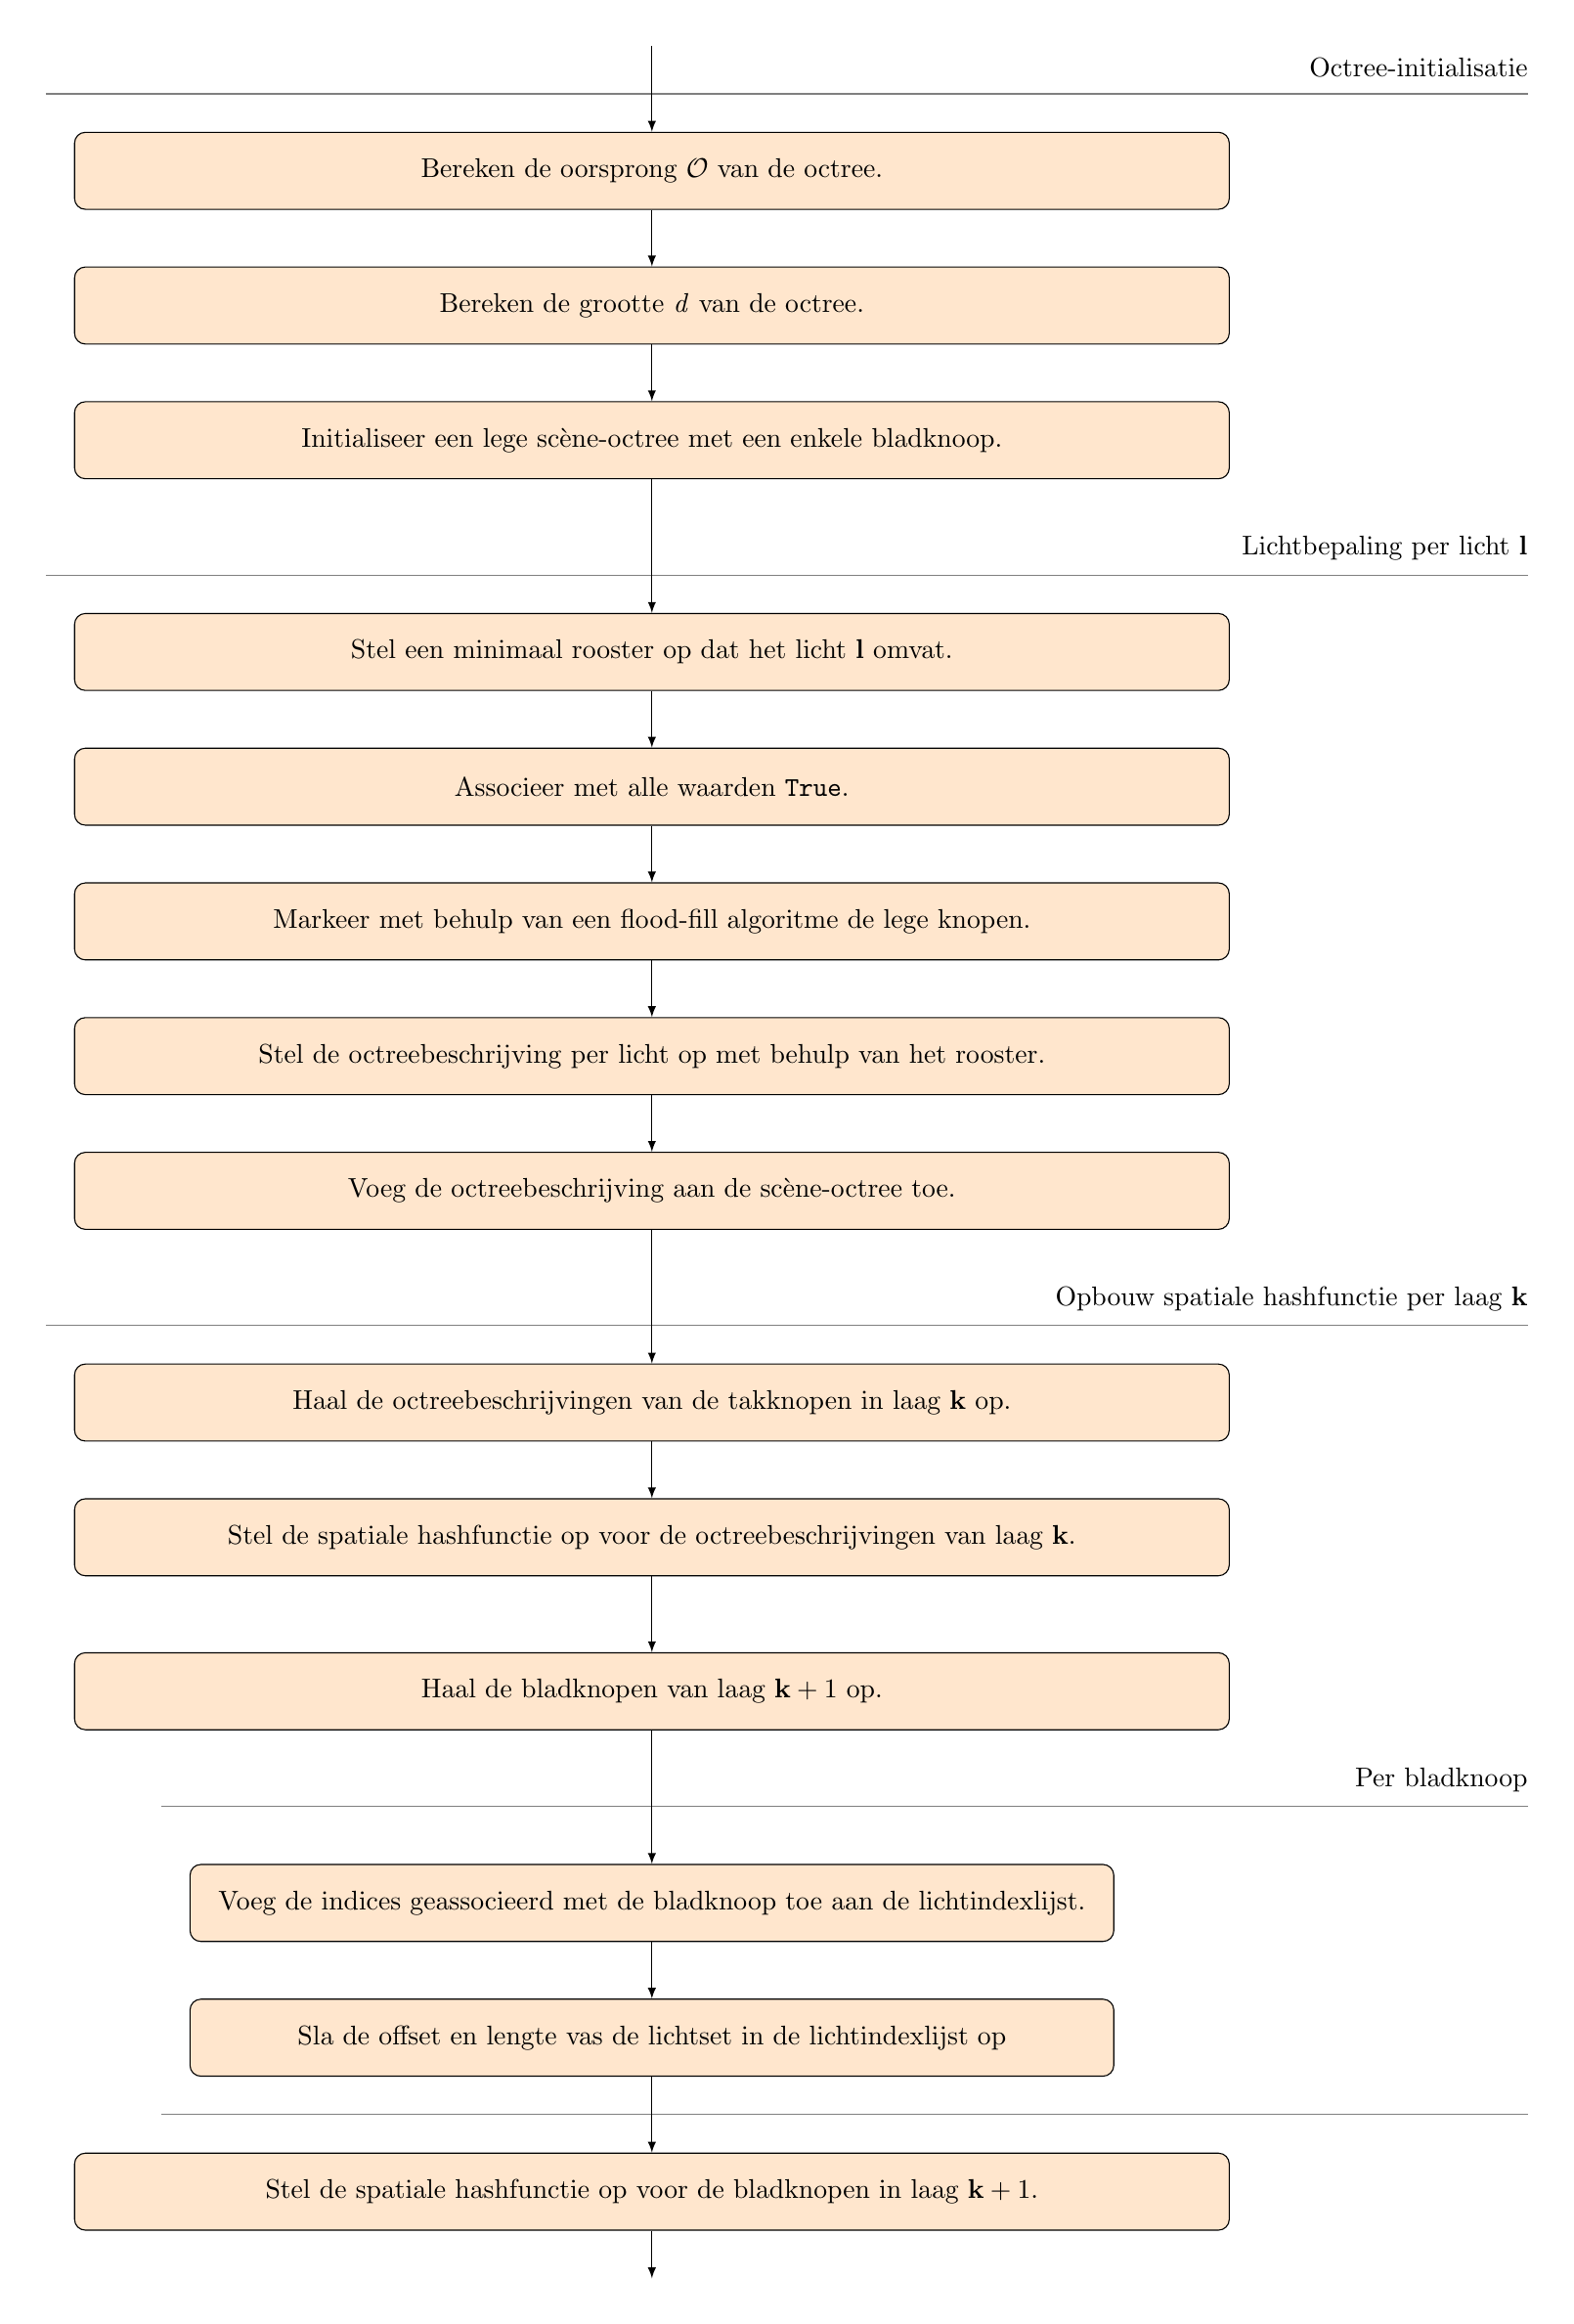
\begin{tikzpicture}[node distance=1.5cm
    every node/.style={fill=white}, align=center]

\node at (0cm, 3cm) (in) [] {};
  \node at (-8cm, 2.25cm) (line1l) [] {};
  \node at ( 11.5cm, 2.25cm) (line1r) [] {};
  \draw[gray] (line1l) -- (line1r);
  \node at (11.5, 2.6) (line1l_t) [anchor=east] {Octree-initialisatie};

\node at (0cm,   1.0cm +0.25cm) (deferred_step0)     [tiled]                  {Bereken de oorsprong $\mathcal{O}$ van de octree.};
\node at (0cm,   -1.0cm + 0.25 * 2cm) (deferred_step1)     [tiled]                 {Bereken de grootte $\mathit{d}$ van de octree.};
\node at (0cm,   -3.0cm + 0.25 * 3cm) (deferred_step2)     [tiled]                 {Initialiseer een lege sc\`ene-octree met een enkele bladknoop.};

  \node at (-8cm, 2.25cm - 7cm  + 0.25 * 3cm) (line1l) [] {};
  \node at ( 11.5cm, 2.25cm - 7cm  + 0.25 * 3cm) (line1r) [] {};
  \draw[gray] (line1l) -- (line1r);
  \node at (11.5cm, 2.6cm - 7cm  + 0.25 * 3cm) (line1l_t) [anchor=east] {Lichtbepaling per licht $\mathbf{l}$};
  
  \node at (0cm,   1.0cm - 7cm  + 0.25 * 4cm) (deferred_step3)     [tiled]                  {Stel een minimaal rooster op dat het licht $\mathbf{l}$ omvat.};
  \node at (0cm,   1.0cm - 7cm - 1 * 2cm  + 0.25cm * 5) (deferred_step4)     [tiled]                  {Associeer met alle waarden $\mathtt{True}$.};
  \node at (0cm,   1.0cm - 7cm - 2 * 2cm  + 0.25cm * 6) (deferred_step5)     [tiled]                  {Markeer met behulp van een flood-fill algoritme de lege knopen.};
  \node at (0cm,   1.0cm - 7cm - 3 * 2cm  + 0.25 * 7cm) (deferred_step6)     [tiled]                  {Stel de octreebeschrijving per licht op met behulp van het rooster.};
  \node at (0cm,   1.0cm - 7cm - 4 * 2cm  + 0.25 * 8cm) (deferred_step7)     [tiled]                  {Voeg de octreebeschrijving aan de sc\`ene-octree toe.};

\node at (-8cm, 2.25cm - 7cm - 5 * 2cm - 1cm + 0.25 * 8cm) (line1l) [] {};
  \node at ( 11.5cm, 2.25cm - 7cm - 4 * 2cm - 1cm) (line1r) [] {};
  \draw[gray] (line1l) -- (line1r);
  \node at (11.5cm, 2.6cm - 7cm - 4 * 2cm - 1cm) (line1l_t) [anchor=east] {Opbouw spatiale hashfunctie per laag $\mathbf{k}$};
  
  \node at (0cm,   1.0cm - 7cm -  4 * 2cm - 1cm + 0.25 * 1cm) (deferred_step8)     [tiled]                  {Haal de octreebeschrijvingen van de takknopen in laag $\mathbf{k}$ op.};
  \node at (0cm,   1.0cm - 7cm -  5 * 2cm - 1cm + 0.25 * 2cm) (deferred_step9)     [tiled]                  {Stel de spatiale hashfunctie op voor de octreebeschrijvingen van laag $\mathbf{k}$.};
  \node at (0cm,   1.0cm - 7cm -  6 * 2cm - 1cm * 1  + 0.25 * 2cm) (deferred_step10)     [tiled]                  {Haal de bladknopen van laag $\mathbf{k} + 1$ op.};
  
  \node at (-6.5cm, 2.25cm - 7cm - 7 * 2cm - 2cm + 0.25 * 3cm) (line1l) [] {};
  \node at ( 11.5cm, 2.25cm - 7cm - 7 * 2cm - 2cm  + 0.25 * 3cm) (line1r) [] {};
  \draw[gray] (line1l) -- (line1r);
  \node at (11.5cm, 2.6cm - 7cm - 7 * 2cm - 2cm  + 0.25 * 3cm) (line1l_t) [anchor=east] {Per bladknoop};
  \node at (0cm,   1.0cm - 7cm -  7 * 2cm - 1cm * 2  + 0.25 * 3cm) (deferred_step11)     [tiled, minimum width=12cm]                  {Voeg de indices geassocieerd met de bladknoop toe aan de lichtindexlijst.};
  \node at (0cm,   1.0cm - 7cm -  8 * 2cm - 1cm * 2 + 0.25 * 4cm) (deferred_step12)     [tiled, minimum width=12cm]                  {Sla de offset en lengte vas de lichtset in de lichtindexlijst op};
  
  \node at (-6.5cm, 2.25cm - 7cm - 9 * 2cm - 2.5cm  + 0.25 * 5cm) (line1l) [] {};
  \node at ( 11.5cm, 2.25cm - 7cm - 9 * 2cm - 2.5cm  + 0.25 * 5cm) (line1r) [] {};
  \draw[gray] (line1l) -- (line1r);
 
\node at (0cm,   1.0cm - 7cm -  9 * 2cm - 1cm * 2.5  + 0.25 * 6cm) (deferred_step13)     [tiled]                  {Stel de spatiale hashfunctie op voor de bladknopen in laag $\mathbf{k} + 1$.};
\node at (0cm,   1.0cm - 7cm -  10 * 2cm - 1cm * 2  + 0.25 * 7cm) (out) [] {};

\draw[-latex] (in) -- (deferred_step0);
\draw[-latex] (deferred_step0) -- (deferred_step1);
\draw[-latex] (deferred_step1) -- (deferred_step2);
\draw[-latex] (deferred_step2) -- (deferred_step3);
\draw[-latex] (deferred_step3) -- (deferred_step4);
\draw[-latex] (deferred_step4) -- (deferred_step5);
\draw[-latex] (deferred_step5) -- (deferred_step6);
\draw[-latex] (deferred_step6) -- (deferred_step7);
\draw[-latex] (deferred_step7) -- (deferred_step8);
\draw[-latex] (deferred_step8) -- (deferred_step9);
\draw[-latex] (deferred_step9) -- (deferred_step10);
\draw[-latex] (deferred_step10) -- (deferred_step11);
\draw[-latex] (deferred_step11) -- (deferred_step12);
\draw[-latex] (deferred_step12) -- (deferred_step13);
\draw[-latex] (deferred_step13) -- (out);

\end{tikzpicture}
\end{adjustbox}
  \caption{Een overzicht van het algoritme om de datastructuren van Hashed Shading op te bouwen.}
  \label{fig:hs-algoritme-beschrijving}
\end{figure}
